\newpage
{\bfseries МРНТИ 06.56.02}

\sectionwithauthors{A. Serikkyzy, A.B. Akhmetova., S.E. Zhamalidenov}{APPROACHES TO MEASURING THE CREATIVE ECONOMY AND TRENDS IN THE
DEVELOPMENT OF THE IT SECTOR: THE IMPACT OF DIGITAL TECHNOLOGIES ON
CREATIVE INDUSTRIES}

\begin{center}
{\bfseries \textsuperscript{1}A. Serikkyzy, \textsuperscript{1}A.B. Akhmetova., \textsuperscript{2}S.E. Zhamalidenov}

\textsuperscript{1}Almaty Management University, Almaty, Kazakhstan,

\textsuperscript{2}Satbayev University, Almaty, Kazakhstan,

Correspondent-author: a.serikkyzy@almau.edu.kz
\end{center}

Today, the creative economy is often referred to a the new oil.
According to UN estimates, creative industries generate around 30
million jobs annually, contributing \$2.25 trillion to the global GDP.
Projections indicate that by 2030, the global creative
industry\textquotesingle s turnover will increase by an additional 40\%.
This sector creates high-income jobs, especially for talented youth.

In Kazakhstan, investments in the creative industry have increased more
than fourfold over the past decade. Currently, 3.5\% of the
country\textquotesingle s total employed population, or 310 thousand
people, work in this sector, contributing 2.7\% to the economy. To
unlock this sector\textquotesingle s potential, the government is
developing the Concept for the Development of Creative Industries for
2021-2025, establishing a unified vision for growth.

The concept of creative industries varies across countries, lacking a
universally accepted definition. Reports like
Australia\textquotesingle s "Creative Nation" (1994) and the
UK\textquotesingle s "Creative Industries Mapping Document" (1998) have
significantly influenced global perspectives. The UN recommends a
classification into four aggregated blocks, but terminology differs
across organizations, with UNESCO using "creative industries" and the EU
referring to "cultural and creative industries."

Creative industries encompass sectors built on creativity, intellectual
property, and technology. Definitions differ, but common sectors include
design, art, fashion, and more. Measuring the creative economy involves
various approaches, such as industry assessment, employment analysis,
and trade in creative goods and services. The "creative trident" concept
evaluates employment in specialists, supporting roles, and integrated
positions.

{\bfseries Keywords}: creative economy, creative industry, investments,
employment, global GDP, technology.

\begin{center}
{\large\bfseries ШЫҒАРМАШЫЛЫҚ ЭКОНОМИКАНЫ ӨЛШЕУ ТӘСІЛДЕРІ ЖӘНЕ IT СЕКТОРЫНЫҢ ДАМУ
ТРЕНДЕНЦИЯЛАРЫ: ЦИФРЛЫҚ ТЕХНОЛОГИЯЛАРДЫҢ ШЫҒАРМАШЫЛЫҚ САЛАЛАРҒА ӘСЕРІ}

{\bfseries \textsuperscript{1}А. Серікқызы, \textsuperscript{1}А.Б.
Ахметова, \textsuperscript{2}С.Е. Жамалиденов}

\textsuperscript{1}Алматы Менеджмент Университеті, Алматы, Қазақстан,

\textsuperscript{2}Satbayev University, Алматы, Қазақстан,

e-mail: a.serikkyzy@almau.edu.kz
\end{center}

Бүгінде жасампаз экономиканы жаңа мұнай деп атайды. Біріккен Ұлттар
Ұйымының бағалауы бойынша, креативті салалар жыл сайын шамамен 30
миллион жұмыс орнын құрып, жаһандық ЖІӨ-ге 2,25 триллион доллар қосады.
Болжамдар 2030 жылға қарай жаһандық креативті индустрияның айналымы тағы
40\%-ға өсетінін көрсетіп отыр. Бұл секторда, әсіресе, талантты жастар
үшін жоғары жалақысы бар жұмыс орындары ашылады.

Қазақстанда шығармашылық индустрияға салынған инвестиция соңғы
онжылдықта төрт еседен астам өсті. Қазіргі уақытта елдегі жалпы жұмыспен
қамтылған халықтың 3,5 пайызы немесе 310 мың адам экономиканың 2,7
пайызын құрайтын осы салада жұмыс істейді. Осы сектордың әлеуетін ашу
үшін үкімет бірыңғай өсу стратегиясын белгілей отырып, 2021-2025
жылдарға арналған Шығармашылық индустрияны дамытудың негізін әзірлеуде.

Шығармашылық индустрия түсінігі әр елде әртүрлі және жаһандық деңгейде
қабылданған анықтамасы жоқ. Австралияның Шығармашылық ұлты (1994) және
Ұлыбританияның Шығармашылық индустрияларды картаға түсіру құжаты (1998)
сияқты есептер жаһандық перспективаларға айтарлықтай әсер етті. БҰҰ төрт
жиынтыққа жіктеуді ұсынады, бірақ терминология ұйымдар арасында
ерекшеленеді, ЮНЕСКО «шығармашылық индустрияларды» пайдаланады, ал ЕО
«мәдени және шығармашылық салаларға» сілтеме жасайды.

Шығармашылық салалар шығармашылыққа, зияткерлік меншікке және
технологияға негізделген секторларды қамтиды. Анықтамалар әртүрлі, бірақ
жалпы секторларға дизайн, өнер, сән және т.б. кіреді. Шығармашылық
экономиканы өлшеу саланы бағалау, жұмыспен қамтуды талдау және
шығармашылық тауарлар мен қызметтердің саудасы сияқты әртүрлі тәсілдерді
қамтиды. Creative Trident тұжырымдамасы мамандардың жұмысқа орналасуын,
көмекші рөлдерді және біріктірілген позицияларды бағалайды.

{\bfseries Түйін сөздер}: креативті экономика, креативті индустрия,
инвестиция, жұмыспен қамту, жаһандық ЖІӨ, технология.

\begin{center}
{\large\bfseries ПОДХОДЫ К ИЗМЕРЕНИЮ КРЕАТИВНОЙ ЭКОНОМИКИ И ТЕНДЕНЦИИ В РАЗВИТИИ
ИТ-СЕКТОРА: ВЛИЯНИЕ ЦИФРОВЫХ ТЕХНОЛОГИЙ НА КРЕАТИВНЫЕ ИНДУСТРИИ}

{\bfseries \textsuperscript{1}А. Серікқызы, \textsuperscript{1}А.Б.
Ахметова, \textsuperscript{2}С.Е. Жамалиденов}

\textsuperscript{1}Алматы Менеджмент Университеті, Алматы, Қазақстан,

\textsuperscript{2}Satbayev University, Алматы, Казахстан,

e-mail: a.serikkyzy@almau.edu.kz
\end{center}

Сегодня креативная экономика часто называется новой нефтью. По оценкам
ООН, креативные отрасли ежегодно создают около 30 миллионов рабочих
мест, внося 2,25 триллиона долларов в мировой ВВП. Прогнозы показывают,
что к 2030 году оборот мировой креативной индустрии увеличится еще на
40\%. Этот сектор создает высокооплачиваемые рабочие места, особенно для
талантливой молодежи.

В Казахстане инвестиции в креативную индустрию выросли более
четырехкратно за последнее десятилетие. В настоящее время в этом секторе
работает 3,5\% от общего числа занятого населения страны, или 310 тысяч
человек, что составляет 2,7\% экономики. Чтобы разблокировать потенциал
этого сектора, правительство разрабатывает Концепцию развития креативных
индустрий на 2021--2025 годы, устанавливая единую стратегию роста.

Концепция креативных индустрий различается в разных странах и не имеет
всемирно признанного определения. Доклады, такие как "Creative Nation"
(1994) Австралии и "Creative Industries Mapping Document" (1998)
Великобритании, значительно повлияли на глобальные перспективы. ООН
рекомендует классификацию на четыре агрегированных блока, но
терминология отличается в различных организациях, с ЮНЕСКО, использующей
"креативные индустрии", а ЕС ссылается на "культурные и креативные
индустрии".

Креативные отрасли охватывают сектора, основанные на творчестве,
интеллектуальной собственности и технологиях. Определения различаются,
но общими секторами являются дизайн, искусство, мода и другие. Измерение
креативной экономики включает различные подходы, такие как оценка
отрасли, анализ занятости и торговля творческими товарами и услугами.
Концепция "креативного трезубца" оценивает занятость специалистов,
поддерживающих ролей и интегрированных позиций.

{\bfseries Ключевые слова}: креативная экономика, креативная индустрия,
инвестиции, занятость, мировой ВВП, технологии.

\begin{multicols}{2}
{\bfseries Introduction.} The concept of creative industries is directly
related to national specificity and varies in each individual country.
There is no universally applied understanding of creative industries
worldwide. Let\textquotesingle s compare the approaches to defining
creative industries that have emerged in different countries. In 1994,
Australia published a report titled "Creative Nation: Cultural Policy of
the Australian Government" (Department of Communications and the Arts
(Australia), 1994). In 1998, the UK Department for Culture, Media and
Sport (DCMS) released the "Creative Industries Mapping Document," the
first major report dedicated to measuring the impact of creative sectors
on the British economy, providing a definition for 13 sectors of
creative industries. This classification significantly influenced the
international economic landscape, drawing attention from policymakers,
and governments embarked on studying the contribution of creativity to
their economies.

The statistical tables of economic indicators for creative industries
published by DCMS include data from all creative sectors, assessing
their contribution to the gross value added of the UK economy. They
consist of three main sections: "Employment," "Gross Value Added," and
"Export Services." The creative industries in these tables are
categorized into the following groups:

- Advertising and marketing;

- Architecture;

- Crafts;

- Design, graphic design, and fashion;

- Film, television, video, broadcasting, and photography;

- Information technology, software, and computer services;

- Publishing;

- Museums, galleries, and libraries;

- Music, performing, and visual arts;

- Video game industry.

The United Nations recommends a classification into four main aggregated
blocks of creative industries, a classification also followed by UNIDO.
Among creative industries are:

- Industries based on the use of historical and cultural heritage (folk
arts and crafts, museum activities);

- Industries based on the arts (theater, music, painting, gallery
activities, etc.);

- Modern media and digital content production (film, video, audio,
animation production, data processing, software development, virtual and
augmented reality, computer and video games, blogging, mass media,
advertising, etc.);

- Applied creative industries (architecture, industrial design, fashion
industry, jewelry making, culinary industry, etc.).

Nevertheless, in international practice, there is no unified definition
and agreed-upon classification of creative industries. UNESCO experts
use the term "creative industries," while at the European Union level,
the term "cultural and creative industries" is applied, and the World
Intellectual Property Organization (WIPO) uses the term "copyright
industries." In some countries, they are still referred to as cultural
industries, while in the Republic of Korea and Japan, they are termed
the content industry. Hence, there are differences in approaches to
measuring and economically assessing creative industries in various
countries, and in some states, such as China, even at the regional and
city levels.

The development of the IT industry in Kazakhstan has seen significant
achievements in recent years, driven by substantial changes and
progress. Kazakhstan aspires to become a technological leader in Central
Asia, and to support this goal, the government has undertaken
initiatives to foster the growth of the IT sector. One such initiative
is the State Program "Digital Kazakhstan", approved by the Government of
the Republic of Kazakhstan on December 12, 2017, through Resolution No.
827 {[}1{]}. In the medium term, the program aims to accelerate economic
development and improve the quality of life through the utilization of
digital technologies, while in the long term, it seeks to create
conditions for transitioning to a digital economy.

The key directions of the State Program "Digital Kazakhstan" include the
development of a creative society and the creation of up to 110,000 new
jobs, transitioning to a proactive state with 80\% of government
services moved online, and implementing digital transformations in
various economic sectors, aiming for up to 5.9\% productivity growth.
The program also envisions the realization of a digital Silk Road to
increase internet users with a coverage of 81.5\% of the population.

In the international Digital Intelligence Index, Kazakhstan ranks 55th
in terms of digitization and 20th in the pace of digitization among 90
countries. In the World Digital Competitiveness Ranking, evaluating the
ability and readiness to implement digital technologies as a key factor
in economic transformations in business, government, and society,
Kazakhstan holds the 36th position out of 63 countries.

As of 2021, the share of the information and communication technology
(ICT) industry in Kazakhstan\textquotesingle s GDP stood at 3.3\%,
according to the Ministry of Digital Development, Innovation, and
Aerospace Industry of the Republic of Kazakhstan (MDDIA). In 2017, this
share was only 1.3\%, and further growth is anticipated by 2023.
According to the National Statistics Bureau, the market volume of
information technology in the ICT industry in Kazakhstan for the first
half of 2021 amounted to 435.66 billion tenge. IT services exceeded IT
equipment by more than twice, reaching 287.46 billion tenge. The IT
services sector is growing in the structure of
Kazakhstan\textquotesingle s IT market, constituting 66.8\%. When
assessing countries with developed digital economies based on the share
of ICT exports in the total volume of goods exports, Kazakhstan lags.
The volume of IT service exports as a percentage of the total export
volume of Kazakhstan in 2022 was 0.1\%. Nevertheless, Kazakhstan has the
potential for development, with a significant internet audience of 17.73
million users, representing 90.9\% of the population. This makes
Kazakhstan an attractive platform for the entry of major international
IT players, providing a new impetus for industry development.

{\bfseries Materials and methods.} The methodological foundation for the
quantitative measurement of creative industries and the creative economy
worldwide has not been definitively established. One of the initial
attempts to classify creative industries was undertaken by the
Department for Culture, Media, and Sport of the United Kingdom in 1998.
Later, UNESCO and UNCTAD proposed alternative typologies {[}2{]}. In
Europe and Asia, creative industries are grouped differently.

One of the current and most debated issues is the measurement of the
creative economy. Attempts to assess the scale of creative industries
and their impact on the national economy are undertaken in many
countries. The most used approaches include:

1. Sectoral Approach: This involves evaluating key economic indicators
based on aggregated groupings of types of economic activities, known as
creative industries.

2. Employment Assessment: This approach involves evaluating employment
based on groupings of professions related to the category of creative
professions.

3. Analysis of External Trade: This entails analyzing international
trade in creative goods and services using relevant statistical
groupings of goods and services, known as creative goods and services.
\end{multicols}

\begin{figure}[H]
	\centering
	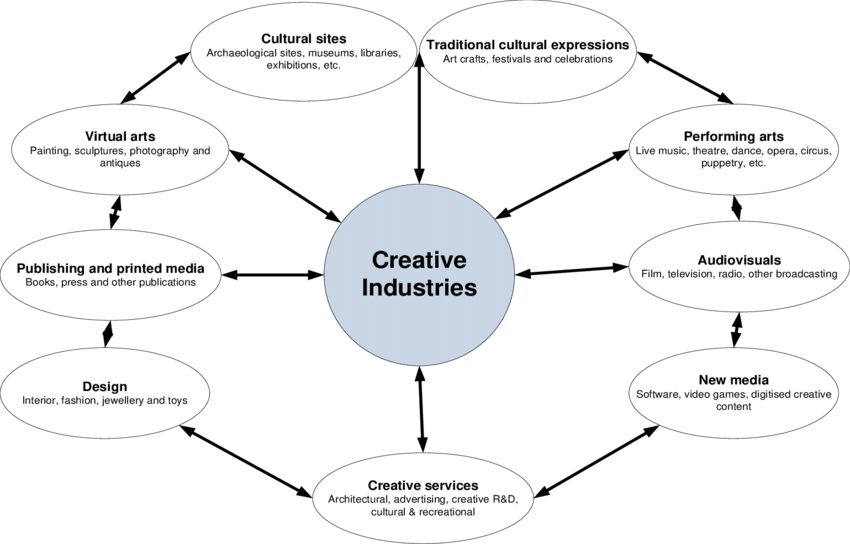
\includegraphics[width=0.8\textwidth]{assets/1120}
	\caption*{Fig. 1 - UNCTAD Classification of Creative Goods {[}2{]}.}
\end{figure}

\begin{multicols}{2}
The creative industries sector has the potential to create high added
value, making it attractive for both entrepreneurs and investors. Many
segments within this sector have relatively low market entry barriers,
providing an opportunity for a broad range of the population to develop
their businesses. This inclusivity extends to women, individuals with
disabilities, people residing in rural areas, and those in small towns,
allowing for widespread participation in the sector\textquotesingle s
growth.

Creative industries make a significant contribution to the global
economy. Over the period from 2002 to 2018, the average share of the
creative industries sector in the world GDP is 6.6\%. In developed
countries, this share reaches 8-12\%, with an average annual growth rate
of 15\%, substantially surpassing the average growth rates of the global
economy.

The creative industries make a substantial contribution to the global
economy. Over the period from 2002 to 2018, the sector has demonstrated
higher growth compared to other industries, generating around 3\% of the
world GDP and providing employment for 1\% of the global working
population. The development of creative industries brings multiple
positive effects to both the economy and society, including the growth
of small and medium-sized enterprises, job creation, diversification,
and an increase in non-commodity exports. It also contributes to
enhancing human capital quality by attracting talents and fostering
in-demand skills. Creative industries serve as a source of sustainable
inclusive growth, providing opportunities for self-development and
creating a conducive environment for living.

The creative economy presents a tangible development option for all
countries, particularly for developing nations. Additional data and
innovative interdisciplinary policy measures are needed to amplify the
impact of the creative sector on development.

The International Year of Creative Economy for Sustainable Development
in 2021 highlights the creative economy at a time when creative
solutions are essential for addressing global challenges {[}3{]}. As
emphasized in UN General Assembly Resolution 74/198 {[}4{]}, the
creative economy contributes comprehensively to achieving Sustainable
Development Goals (SDGs), especially Goals 1 (poverty eradication), 5
(gender equality), 8 (decent work and economic growth), 9 (industry,
innovation, and infrastructure), 10 (reduced inequality), 11
(sustainable cities), 12 (responsible consumption and production), 16
(peaceful and inclusive societies), and 17 (partnerships for the goals).

Cultural and creative industries undeniably make a significant
contribution to the global economy. The cultural sector accounts for
3.1\% of the world\textquotesingle s Gross Domestic Product (GDP), while
creative goods and services comprised 3\% and 21\%, respectively, of the
total volume of goods and services exports in 2020, according to UNCTAD
estimates {[}5{]}. Additionally, cultural, and creative industries
provide 6.2\% of all jobs worldwide, nearly 50 million, with a higher
representation of young people (15--29 years) compared to other sectors.
The creative economy promotes social inclusion, cultural diversity, and
human development. For these reasons, creative industries are crucial
for achieving the 2030 agenda. However, the COVID-19 pandemic has had a
devastating impact on some creative sectors, exacerbating longstanding
factors contributing to their vulnerability. A UNCTAD report indicates
that during this period, up to 10 million jobs disappeared in the
cultural and creative sectors, and in 2020, global production in these
sectors decreased by USD 750 billion {[}2{]}.

{\bfseries Results and discussion}.Analyzing the key aspects of the IT
industry in Kazakhstan, several development trends can be highlighted:

1. Economic Growth and Investments. In Kazakhstan, a favorable
environment has been established for investments in the IT sector. The
government actively supports startups and technology companies by
providing tax incentives and other stimuli. This approach attracts both
local and foreign investments into the markets. According to the
National Statistics Bureau of the Agency of Statistics of the Republic
of Kazakhstan, the IT market volume in 2022 amounted to 1.71 million
dollars, with a growth of 40.3\% in the ICT industry. The sector employs
69.5 thousand workers. The total capitalization of foreign technological
giants that relocated to Kazakhstan in 2022 reached 27 billion dollars
{[}6{]}. In 2020, the export of ICT goods and services amounted to
approximately 73.6 million US dollars, with ICT services contributing
more than 24 million US dollars. Over 50\% of service exports are
directed to European countries and the United States.

2. Training and Skill Development Programs. The development of the IT
industry in Kazakhstan involves the creation of educational programs and
courses focusing on software development, data analysis, and other
IT-related fields. The majority of IT specialists still receive
traditional education, completing bachelor\textquotesingle s and
master\textquotesingle s degrees. Currently, 84 out of 116 higher
education institutions provide training for information technology
professionals. Annually, 8,000 to 9,000 educational grants are allocated
for the preparation of IT specialists. The number of graduates from 2018
to 2020 reached 30,604. However, according to experts and market
participants, not more than 30\% of graduates possess the necessary
skills for a successful career in their field, as indicated by the
National Chamber of Entrepreneurs "Atameken" rating {[}7{]}.

Кazakhstan universities and training centers provide opportunities for
education and skills enhancement in the IT field. According to a survey
conducted by Kolesa Group {[}8{]}, 78\% of respondents studied IT
specialties at three major universities in the country -- International
IT University (17\%), SDU University (10\%), and Almaty University of
Power Engineering and Telecommunications (7\%).

The most in-demand IT specialists in Kazakhstan are:

1. Programmer, Developer.

2. Designer.

3.Analyst.

4. System Administrator.

5. Technical Support Specialist.

6. Information Security Specialist.

7. Systems Engineer.

8. Tester.

9. Network Engineer.

10. Game Designer.

Around 21\% of IT specialists in Kazakhstan officially work for at least
two companies. Since 2021, there has been a trend towards obtaining
education not only in universities but also through specialized
programs, allowing individuals to acquire specific skills and enhance
hard skills in a short period. For instance, in 2022, Tech Orda from
Astana Hub graduated 3,000 individuals, and alem.school trained 250
specialists through educational IT programs. The International Financial
Center "Astana" and Qwazar jointly launched the QWANT programming
school, currently educating 250 Kazakhstani and international
specialists.

According to digitalbusiness.kz {[}9{]}, the IT sector ranked fifth in
the rating of open job vacancies in Kazakhstan. In Q1 and Q2 of 2023,
more than 50,000 residents of Kazakhstan were searching for jobs in the
information technology sector. In 2022, about 40,000 IT job vacancies
were published, constituting 48\% of all job postings, according to the
hh.kz platform.

The high interest in IT specialties in Kazakhstan is driven by
competitive salaries in the IT sector, company bonuses, the development
of artificial intelligence, and the emergence of new innovative products
in the IT industry. According to hh.kz data, the salary for a leading
DevOps engineer and Java- and iOS-developers varies from 700,000 to 2.3
million tenge, with the average salary for an IT specialist in 2022
reaching 515,600 tenge {[}8{]}.

3. Startup Ecosystem. The startup ecosystems in Kazakhstan are actively
evolving. Incubators, accelerators, and technoparks have been
established to foster the digital sector and support young
entrepreneurs, contributing to the development of innovations and new
technological projects. Some of the largest ones include:

- International Financial Center Astana: A cluster with over 1,700
registered companies, attracting investments of \$7.4 billion.

- Astana Hub: A technopark for startups with favorable tax conditions.
By the end of 2022, nearly a thousand IT companies were participants in
Astana Hub.

- MOST Business Incubator: A business incubator that has helped attract
over \$6 million in investments to startups.

4. Software Development. Kazakhstani IT companies continue to develop
software for various sectors, including banking, logistics, government
administration, and more. Exporting software solutions is a lucrative
business. However, the accelerated pace of digitization worldwide will
lead to a shortage of developers. By 2025, it is projected to reach 17
million specialists8. This shortage may arise due to the growth of
complex projects in AI, data analytics, and similar fields.
Universities, courses, and training programs may struggle to produce a
sufficient number of tech specialists capable of supporting innovation
in technology companies. In turn, junior specialists may not be
adequately prepared to tackle complex tasks, and the demand for their
skills will continue to grow each year. The main challenge lies in the
fact that the level of education does not align with the business needs
and lags behind in development.

5. E-Government and Digitization. Kazakhstan is actively integrating
technologies into public administration. In 2020, the country ranked
29th out of 193 nations in the UN E-Government Development Index,
marking a rise of 10 positions {[}10{]}.

The Electronic government of the Republic of Kazakhstan has been
operational since 2006. The project is part of the
government\textquotesingle s "Digital" initiatives, led by the
Ministries of Justice, Digital Development, Innovations, and Aerospace
Industry, in collaboration with the National Information Technologies
JSC.

The Electronic government of the Republic of Kazakhstan enables citizens
and businesses to interact with the government online, ensuring the
delivery of quality services and reducing bureaucracy. Out of 45 types
of government services, 43 services, or 95\%, can be obtained in
electronic format, including 23 services proactively (51\%) {[}11{]}. In
2022, a total of 13.8 million government services were provided, with
11.2 million being electronic services, accounting for 81\% of the total
number of services rendered {[}11{]}.

6. Artificial Intelligence and Analytics. In Kazakhstan, the field of
artificial intelligence is actively advancing. The application of AI
involves data analysis for decision-making in various sectors, ranging
from healthcare to business. Investments in data processing and storage
will increase sixfold in Kazakhstan, from 82 billion to 500 billion
tenge {[}10{]}. The development of AI and automation will impact the
labor market, potentially leading to the emergence of new professions or
the reduction of existing ones. About 29\% of tasks performed by humans
with a high or moderate likelihood can be automated, and 13\% of tasks
can be handled by AI {[}12{]}.

7. Cybersecurity. With the advent of digital technologies, the level of
cybersecurity is also increasing. Kazakhstan is developing strategies
and measures to ensure the protection of data and information
activities. According to the Global Cybersecurity Index, which assesses
the cybersecurity level of countries, Kazakhstan made a significant
improvement in 2018, rising from the 83rd to the 40th position in just
one year {[}13{]}. Among the Commonwealth of Independent States (CIS),
Kazakhstan secured the second position after Russia. In 2017, the
cybersecurity concept "Cyber Shield of Kazakhstan" was approved, and in
2022, the "Cyber Shield-2" Concept for the development of the digital
ecosystem for 2022-2027 was introduced {[}14{]}. This concept outlines
key directions for implementing state policies in the IT and
telecommunications sector, protecting electronic information resources,
and ensuring the security of information and communication technologies
usage.

The development of the IT industry in Kazakhstan is ongoing, and the
country is actively working on creating an innovative and competitive
ecosystem that contributes to economic growth and technological
progress. In recent years, Kazakhstan has also started paying attention
to sustainable development and responsibility in the information
technology sector, addressing issues such as energy efficiency and
carbon footprint reduction. Kazakhstan is developing and implementing a
strategy for the development of information and communication
technologies, outlining priority directions and goals for the IT
industry.

The core of the definition of creativity lies in the interaction of
human creativity, ideas, intellectual property, knowledge, and
technology; the creative economy encompasses all industries built on
creative activity. The concept of the creative economy is closely
related to the "knowledge economy," a key factor in organic growth
through investments in human capital.

Definitions significantly differ between countries and international
organizations. For example, the Inter-American Development Bank (IDB)
defines the creative (or yellow) economy as "a group of activities in
which ideas are transformed into cultural and creative goods and
services that enjoy or can enjoy protection as intellectual property"
{[}15{]}.

According to the approaches of the United Nations Educational,
Scientific and Cultural Organization (UNESCO), creative industries
involve the creation, production, and commercialization of goods and
services primarily based on the use of intellectual activity results.
UNESCO pays special attention to the socio-economic aspects of culture,
defined in accordance with concepts of cultural and related domains and
the cultural cycle {[}16{]}.

United Nations Conference on Trade and Development (UNCTAD) defines
creative industries as cycles of creation, production, and distribution
of goods and services where creativity and intellectual capital are used
as the primary resources {[}17{]}. They encompass a set of
knowledge-based activities to produce tangible goods and intangible
intellectual or artistic services with a creative component and economic
value, intended for sale in the market.

In Russian sources, "creative industries" is understood as an economic
sector that includes interdependent and interpenetrating industries in
the fields of research, development, and production of goods and
services originating in individual creativity, skills, and talents.
These industries have the potential for enrichment and job creation
through the creation and use of intellectual property {[}18{]}.

The same understanding of creative industries is defined in Kazakhstan
in the "Concept for the Development of Creative Industries for
2021-2025" {[}19{]}. Creative industries encompass economic sectors
whose raw materials are imagination, creativity, and intellectual
capital. In addition to traditional sectors of the economy associated
with the classical understanding of culture and arts, creative
industries can also include the digital sector, professional, scientific
and technical activities, and the information and communication sector.

According to the current United Nations approaches, creative industries
encompass 14 sectors, including design, art, fashion, film, music,
media, computer graphics, education, and other areas based on
intellectual activity. In international practice, creative industries
encompass over two thousand types of activities.

One of the current and most debated challenges is the measurement of the
creative economy. Many countries are attempting to assess the scale of
creative industries and their impact on the national economy. Among the
most used approaches are:

1. Industry approach, which involves evaluating key economic indicators
based on aggregated groupings of types of economic activities (creative
industries).

2. Employment assessment based on groupings of professions related to
the category of creative (creative professions).

3. Analysis of foreign trade in creative goods and services using
relevant statistical groupings of goods and services (creative goods and
services).

The initial attempts to measure the creative economy were based on an
industry approach, which relies on defining a list of economic
activities related to "creative" sectors. This methodology faced
significant criticism from the outset for various objective reasons,
such as:

- The lack of clear criteria for the "creativity" of industries.

- Frequent discrepancies between officially declared and actual
activities of organizations.

- Incomplete information about individual entrepreneurs, self-employed
individuals, and those working in the "unobserved" economy.

Despite these shortcomings, the industry approach remains the most
common to date, as it allows for the assessment of key economic
indicators of creative industries. Many countries and cities actively
implement their own industry classifications. To ensure data
comparability, these classifications generally draw on international
approaches and recommendations (UNESCO, WIPO, among others) while also
considering the priorities of national or regional policies.
\end{multicols}

\begin{table}[H]
\caption*{Table 1 - UNCTAD Classification of Creative Goods}
\centering
\begin{tabular}{|l|l|}
\hline
Art Crafts & Audiovisuals \\ \hline
\begin{tabular}[c]{@{}l@{}}- Holiday items\\ - Other art crafts\\ - Hand-cast paper and cardboard\\ - Woven products\\ - Wicker products\end{tabular} & \begin{tabular}[c]{@{}l@{}}- Kinofilm  \\ - Magnetic media\end{tabular} \\ \hline
Design & New Media \\ \hline
\begin{tabular}[c]{@{}l@{}}- Architectural and design projects\\ - Fashion accessories\\ - Glass products\\ - Interior items\\ - Jewelry\\ - Games and toys\end{tabular} & \begin{tabular}[c]{@{}l@{}}- Information recorded carriers\\ - Goods for video games\end{tabular} \\ \hline
Visual Arts & Publishing \\ \hline
\begin{tabular}[c]{@{}l@{}}- Collectibles and antiques\\ - Painting\\ - Photography\\ - Sculpture\end{tabular} & \begin{tabular}[c]{@{}l@{}}- Books\\ - Newspapers\\ - Other printed products\end{tabular} \\ \hline
Performing Arts &  \\ \hline
\begin{tabular}[c]{@{}l@{}}- Musical instruments\\ - Sheet music\end{tabular} &  \\ \hline
\end{tabular}
\end{table}

\begin{multicols}{2}
"Employment Assessment in Creative Professions - an alternative approach
to measuring the scale of the creative economy of a city. It is based on
the classification of occupations related to the creative field.
Calculations use data from selective labor force surveys conducted in
many countries. In the assessment, the concept of the
\textquotesingle creative trident\textquotesingle{} is often applied,
where three groups of individuals working in the creative sphere are
identified {[}20{]}:

- Employed in creative professions in creative industries
(\textquotesingle specialists\textquotesingle);

- Employed in other professions in creative industries
(\textquotesingle supporting\textquotesingle);

- Employed in creative professions in other sectors
(\textquotesingle integrated\textquotesingle). The sum of the three
mentioned categories of workers is considered as a consolidated
characteristic of employment in the creative economy. The analysis of
the \textquotesingle integrated\textquotesingle{} category allows for an
evaluation of the extent of the penetration of creative professions into
other industries."

Another recognized approach to studying the creative economy is the
analysis of trade in creative goods and services. Statistical standards
in this area are set by the United Nations Conference on Trade and
Development (UNCTAD). Creative goods constitute a broad category of
tangible products that can be produced on both an individual and mass
scale, crafted by hand or manufactured using modern industrial
equipment. They have both aesthetic and functional value. These goods
are created, produced, and distributed for commercial purposes while
possessing creative content, economic, and cultural value {[}21{]}.
Based on these criteria and the Harmonized System for the Description
and Coding of Goods by the World Customs Organization, seven broad
groups of creative goods are identified {[}22{]}.

{\bfseries Сonclusion.} The concept of creative industries is directly
related to national specificity and varies in each individual country.
There is no universally applied understanding of creative industries
worldwide. For instance, in 1994, Australia published "Creative Nation:
Cultural Policy of the Australian Government," and in 1998, the UK
Department for Culture, Media and Sport (DCMS) released the "Creative
Industries Mapping Document," which defined 13 sectors of creative
industries. These classifications have significantly influenced the
international economic landscape, prompting governments to study the
contribution of creativity to their economies.

In Kazakhstan, the development of the IT industry has seen significant
achievements driven by substantial changes and progress. The government
aims to position Kazakhstan as a technological leader in Central Asia,
supporting this goal with initiatives like the State Program "Digital
Kazakhstan," approved on December 12, 2017. This program aims to
accelerate economic development and improve the quality of life through
digital technologies, with long-term goals of transitioning to a digital
economy.

However, the sector faces several challenges:

1. Lack of Developed Infrastructure: 85\% of entrepreneurs require
workspaces, emphasizing the importance of synergy from co-location
despite remote work opportunities.

2. Low Business Management Competencies: 56\% of entrepreneurs need
training in creative entrepreneurship, especially in crafting business
plans, defining business strategies, and managing accounting and tax
records.

3. Inaccessibility of Preferential Financing: 31\% of entrepreneurs cite
insufficient funding, with 35\% unaware of existing state support
instruments despite programs like Almaty Business -- 2025 and the
``Damu'' Entrepreneurship Development Fund.

4. Shortage of Qualified Personnel: 10\% of entrepreneurs identify a
shortage of skilled workforce, especially in IT areas like artificial
intelligence and cloud computing.

5. Lack of Export Support Programs: To scale and enter international
markets, creative entrepreneurs require support from funds and private
investors, assistance in finding sales agents, and development of
contacts with creative entrepreneurs in other countries.

Despite these challenges, the IT market in Kazakhstan demonstrates high
growth potential. The country has a substantial internet audience, an
increasing share of ICT in the overall GDP, and conditions are being
created for the entry of major international IT players. The sector is
marked by a growing share of educational IT programs and more people
seeking employment in IT. However, there is a need to prevent IT talents
from migrating abroad by creating conducive conditions for work and
career development within Kazakhstan.

The information and IT industry plays a pivotal role in contemporary
realities, providing means for information exchange and facilitating
communication between individuals and organizations. Increasing
technological demands and the constant evolution of digital tools make
this industry critically important for numerous sectors, including
business, science, education, entertainment, and creative industries.

There are several prospects and potential impacts of information
technology on the development of creative industries:

- Expansion of Access to Creativity: IT technologies provide numerous
platforms and tools for creating, distributing, and accessing creative
content, allowing creative individuals to showcase their work to a wide
audience.

- Improvement of Content Production and Distribution: Information
technologies optimize the processes of producing and distributing
cultural products, reducing costs and increasing efficiency.

- Cultural Exchange and Collaboration: Global networks and
content-sharing platforms enable artists and creative collectives to
collaborate and interact across different parts of the world, fostering
cultural exchange.

- Virtual and Augmented Realities: These technologies open new horizons
for creative industries, allowing the creation of innovative and unique
visual and interactive formats.

- Digital Distribution and Marketing: Information technology facilitates
effective digital distribution and marketing of creative products,
reaching a broader audience beyond territorial boundaries.

- Analytics and Artificial Intelligence: The use of data analytics and
AI in creative industries can help predict demand for content and adapt
it to the audience\textquotesingle s needs, significantly altering the
industry\textquotesingle s development.

In summary, the IT and creative sectors in Kazakhstan are interlinked
and vital for the country\textquotesingle s economic growth. The
development of these sectors not only enhances the quality and
efficiency of creative content production but also broadens its
influence and accessibility to a wide audience, contributing to the
development and prosperity of creative industries. Addressing the
challenges of infrastructure, financing, skill shortages, and export
support is crucial for maximizing the potential of these industries.
\end{multicols}

\begin{center}
{\bfseries References}
\end{center}

\begin{noparindent}
1.Postanovlenie Pravitel\textquotesingle stva Respubliki Kazakhstan ot
12 dekabrya 2017 goda № 827. Ob utverzhdenii

Gosudarstvennoi programmy
  "Tsifrovoi Kazakhstan". -URL:
  https://adilet.zan.kz/rus/docs/P1700000827. (data obrashcheniya:
  28.05.2024)

2.The 2009 UNESCO framework for cultural statistics (FCS). --UNESCO
  Unstitute for Statistics, 2009. -98 p. ISBN 978-92-9189-075-0

3.UNESCO: International Year of Creative Economy for Sustainable
  Development. - URL:

  https://www.unesco.org/en/articles/international-year-creative-economy-sustainable-development
  (Date of

  application - 28.05.2024)

4.UN trade\& development: International Year of Creative Economy for
  Sustainable Development, 2021. -URL:
  https://unctad.org/topic/trade-analysis/creative-economy-programme/2021-year-of-the-creative-economy
  (date of application: 28.05.2024)

5.Technology and innovation report 2021. --UNITED NATIONS, Geneva, 2021.
  ISBN: 978-92-1-113012-6 --URL:
  https://unctad.org/system/files/official-document/tir2020\_en.pdf
  (date of application: 28.05.2024)

6.Inbusiness.kz: Skol\textquotesingle ko stoyat IT-spetsialisty v
  Kazakhstane? URL:
  https://inbusiness.kz/ru/news/skolko-stoyat-it-specialisty-v-kazahstane
  (date of application: 28.05.2024) {[}in Russian{]}

7.Postanovlenie Pravitel\textquotesingle stva Respubliki Kazakhstan ot
  30 dekabrya 2021 goda № 961. Ob utverzhdenii Kontseptsii razvitiya
  otrasli informatsionno-kommunikatsionnykh tekhnologii i tsifrovoi
  sfery. --URL:

  https://adilet.zan.kz/rus/docs/P2100000961 (data
  obrashcheniya: 28.05.2024) {[}in Russian{]}

8.Astana Hub: 8 trendov, kotorye opredelyayut IT-rynok v Kazakhstane.
  -2023.
  https://astanahub.com/ru/blog/8-trendov-kotorye-opredeliaiut-it-rynok-v-kazakhstane
  (data obrashcheniya: 28.05.2024)

9.Digital Business: V HeadHunter prognoziruyut, chto v 2023 godu po
  chislu vakansii sfera informatsionnykh tekhnologii stanet liderom v
  Kazakhstane. -2022. --URL:
  https://digitalbusiness.kz/2022-12-03/v-headhunter-prognoziruyut-chto-v-2023-godu-po-chislu-vakansij-sfera-informaczionnyh-tehnologij-stanet-liderom-v-kazahstane/
  (date obrashcheniya: 28.05.2024) {[}in Russian{]}

10.The Press Service of the Government of the Republic of Kazakhstan
  (2021). Kazakhstan took 29th place in the UN rating on e-government
  development. --URL:
  https://primeminister.kz/en/news/kazakstan-elektrondyk-ukimetti-damytu-dengeyi-boyynsha-buu-reytinginde-29-oryn-aldy-515451
  (date of application: 28.05.2024)

11.The Press Service of the Government of the Republic of Kazakhstan
  (2023). 2.4 million state services in electronic format received by
  Kazakhstan in the first quarter of 2023. --URL:
  https://primeminister.kz/en/news/reviews/24-million-state-services-in-electronic-format-received-by-kazakhstan-in-the-first-quarter-of-2023-23879
  (date of application: 28.05.2024)

12. Ministerstvo truda i sotsial\textquotesingle noi zashchity naseleniya
Respubliki Kazakhstan: Vliyanie avtomatizatsii i iskusstvennogo
intellekta na rynok truda v Kazakhstane otsenili v TsRTR. --URL:

https://www.gov.kz/memleket/entities/enbek/press/news/details/579455?lang=ru
(data obrashcheniya: 28.05.2024) {[}in Russian{]}

13. FinProm: Kolichestvo intsidentov, svyazannykh s atakami i ugrozami
informatsionnoi bezopasnosti, sokratilos\textquotesingle{} v sravnenii s
proshlym godom na 23\%. -2019. --URL:
https://finprom.kz/ru/article/kolichestvo-incidentov-svyazannyh-s-atakami-i-ugrozami-informacionnoj-bezopasnosti-sokratilos-v-sravnenii-s-proshlym-godom-na-23
(data obrashcheniya: 28.05.2024) {[}in Russian{]}

14. Zakon.kz: Kontseptsiya razvitiya tsifrovoi ekosistemy na 2022-2027 goda
(«Kibershchit-2»). -2022. --URL:
https://online.zakon.kz/Document/?doc\_id=31786606\&pos=6;-106\#pos=6;-106
(data obrashcheniya: 28.05.2024) {[}in Russian{]}

15. Benavente José Miguel. Public policies for creativity and innovation:
promoting the orange economy in Latin America and the Caribbean / José
Miguel Benavente, Matteo Grazzi// Inter-American Development Bank.
-6017. DOI 10.18235/0000841

17. The 2009 UNESCO Framework for Cultural Statistics (FCS)// UNESCO
Institute for Statistics. - Montreal~:~UNESCO-UIS,~2009. -98 p. ISBN
978-92-9189-075-0

18.Creative Economy Outlook // UCTAD. -New York, 2022. ISBN:
  978-92-1-113072-0

19.Atlas kreativnykh industrii Rossiiskoi Federatsii. -2021. -555 s.
  {[}in Russian{]}

20. Postanovlenie Pravitel\textquotesingle stva Respubliki Kazakhstan ot
  30 noyabrya 2021 goda № 860 Ob utverzhdenii Kontseptsii razvitiya
  kreativnykh industrii na 2021 - 2025 gody. --URL:
  https://online.zakon.kz/Document/?doc\_id=33480048. (data
  obrashcheniya: 28.05.2024) {[}in Russian{]}

21. Higgs P., Cunningham S. Australia's Creative Economy: Mapping
  Methodologies. -Technical Report. Brisbane: CCI, 2007. --URL:
  https://eprints.qut.edu.au/225658/1/6228.pdf. (date of application -
  28.05.2024)

22. Creative Economy Outlook: Trends in international trade in creative
  industries. -United Nations. 2018. --URL:
  https://unctad.org/system/files/official-document/ditcted2018d3\_en.pdf
  (дата обращения: 28.05.2024)

23. UNCTAD: Creative goods groups (HS 2007)

  https://unctadstat.unctad.org/EN/Classifications/DimHS2007Products\_Creatives\_Hierarchy.pdf
  (date of application - 28.05.2024)
\end{noparindent}

\emph{{\bfseries Information about the authors}}

\begin{noparindent}
Serikkyzy A.- PhD, associate professor Almaty management university
ALMAU, Almaty, Kazakhstan, e-mail: a.serikkyzy@almau.edu.kz;

Akhmetova A.B.-student of ALMAU, Almaty, Kazakhstan, e-mail:
akh.a@gmail.com;

Zhamalidenov S. E.-master student of Satbayev University, Almaty,
Kazakhstan, e-mail: s.zhamalidenov@mail.ru.
\end{noparindent}

\emph{{\bfseries Сведения об авторах}}

\begin{noparindent}
Серіккызы А. -PhD, ассоциированный профессор ALMAU, Аламаты, Казахстан,
e-mail: a.serikkyzy@almau.edu.kz;

Ахметова А. Б. - студент ALMAU,Аламаты, Казахстан, e-mail:
akh.a@gmail.com;

Жамалиденов С. Е.- магистрант Satbayev University, Алматы, Казахстан,
e-mail: s.zhamalidenov@mail.ru.
\end{noparindent}
